\documentclass[tikz,border=10pt]{standalone}
\usetikzlibrary{positioning, fit, shapes.multipart}

\begin{document}
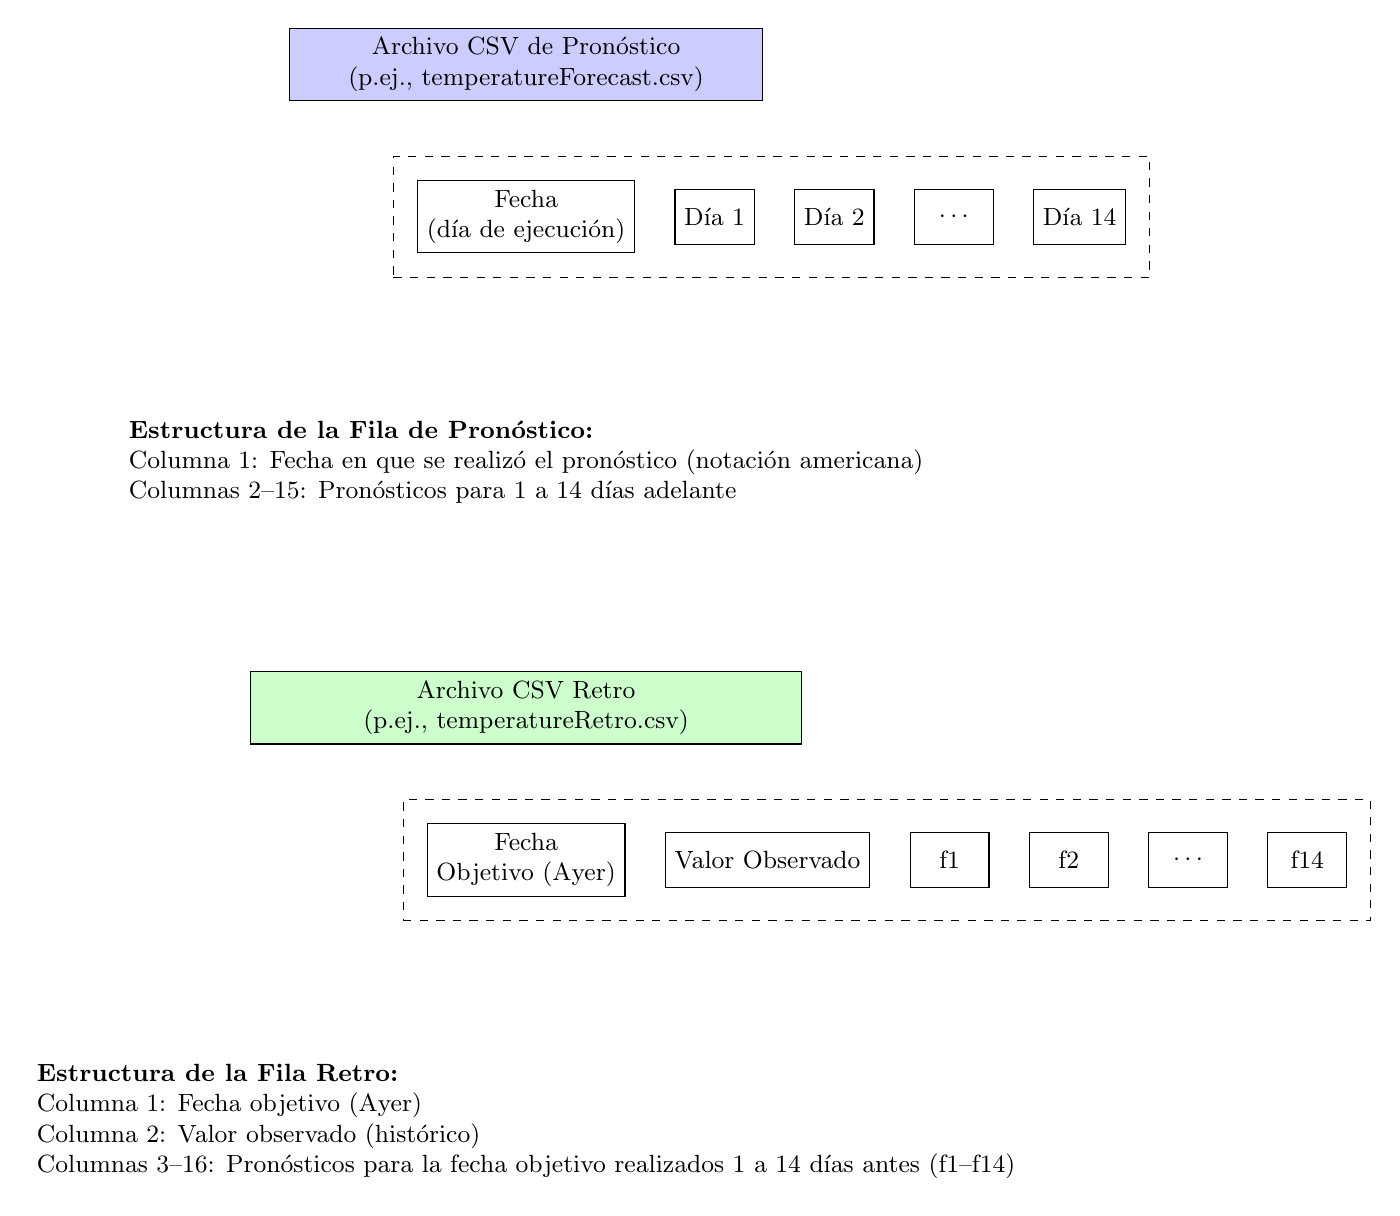
\begin{tikzpicture}[
    node distance=1.0cm and 0.5cm,
    every node/.style={font=\small},
    encabezado/.style={rectangle, draw, fill=gray!20, minimum width=1cm, minimum height=0.7cm, align=center},
    celda/.style={rectangle, draw, minimum width=1cm, minimum height=0.7cm, align=center}
  ]
  
  % ---------------- Archivo CSV de Pronóstico ----------------
  \node (tituloPron) [encabezado, fill=blue!20, minimum width=6cm] {Archivo CSV de Pronóstico\\(p.ej., temperatureForecast.csv)};
  
  % Fila de pronóstico: 15 columnas
  \node (pc1) [celda, below=of tituloPron] {Fecha\\(día de ejecución)};
  \node (pc2) [celda, right=of pc1] {Día 1};
  \node (pc3) [celda, right=of pc2] {Día 2};
  \node (pc4) [celda, right=of pc3] {$\cdots$};
  \node (pc5) [celda, right=of pc4] {Día 14};
  
  % Dibujar un recuadro alrededor de la fila (opcional)
  \node [draw, dashed, fit=(pc1) (pc5), inner sep=3mm] {};
  
  % Nota explicativa
  \node (notaPron) [below=of pc1, yshift=-1cm, align=left] {
    \textbf{Estructura de la Fila de Pronóstico:}\\
    Columna 1: Fecha en que se realizó el pronóstico (notación americana)\\
    Columnas 2--15: Pronósticos para 1 a 14 días adelante
  };
  
  % ---------------- Archivo CSV Retro ----------------
  \node (tituloRetro) [encabezado, fill=green!20, minimum width=7cm, below=of notaPron, yshift=-1cm] {Archivo CSV Retro\\(p.ej., temperatureRetro.csv)};
  
  % Fila retro: 16 columnas
  \node (rc1) [celda, below=of tituloRetro] {Fecha\\Objetivo (Ayer)};
  \node (rc2) [celda, right=of rc1] {Valor Observado};
  \node (rc3) [celda, right=of rc2] {f1};
  \node (rc4) [celda, right=of rc3] {f2};
  \node (rc5) [celda, right=of rc4] {$\cdots$};
  \node (rc6) [celda, right=of rc5] {f14};
  
  % Dibujar un recuadro alrededor de la fila retro (opcional)
  \node [draw, dashed, fit=(rc1) (rc6), inner sep=3mm] {};
  
  % Nota explicativa
  \node (notaRetro) [below=of rc1, yshift=-1cm, align=left] {
    \textbf{Estructura de la Fila Retro:}\\
    Columna 1: Fecha objetivo (Ayer)\\
    Columna 2: Valor observado (histórico)\\
    Columnas 3--16: Pronósticos para la fecha objetivo realizados 1 a 14 días antes (f1--f14)
  };
  
\end{tikzpicture}
\end{document}
